\newcommand{\institut}{Institut f\"ur Energie und  Automatisiertungstechnik}
\newcommand{\fachgebiet}{Elektronische Mess- und Diagnosetechnik}
\newcommand{\veranstaltung}{Praktikum Messdatenverarbeitung}
\newcommand{\pdfautor}{\"Ozg\"u Dogan (326 048), Timo Lausen (325 411), Boris Henckell (325 779)}
\newcommand{\autor}{\"Ozg\"u Dogan (326 048)\\ Timo Lausen (325 411)\\ Boris Henckell (325 779)}
\newcommand{\pdftitle}{Praktikum Messdatenverarbeitung  Termin 1}
\newcommand{\prototitle}{Praktikum Messdatenverarbeitung \\ Termin 1}
\newcommand{\aufgabe}{}

\newcommand{\gruppe}{Gruppe: G1 Fr 08-10}
\newcommand{\betreuer}{Betreuer: J\"urgen Funk}

\input{../../packages/tu_header_8}
%---------------------------------------------------------------------
%---------------------------------------------------------------------
%---------------------------------------------------------------------

\section{Vorbereitungsaufgaben}
\begin{quote}
    \subsection{Stellen Sie Ihre Implementierung des Interruptgesteuerten ADUs fertig.}
    \begin{quote}
        siehe Protokoll vom Termin 1
    \end{quote}
    
	\subsection{Aufbau digitale Messkette}
    \begin{quote}
        Eine Digitale Messkette dient dem Zweck ein analoges Signal mit Hilfe eines Sensors zu erfassen und in ein
        Digitales Signal umzuwandeln.\\
        Konkret werden für die Messkette folgende Bauteile benötigt:
        \begin{itemize}
          \item Sensor
          \item Signalkonditionierung
          \item Anti-Aliasingfilter
          \item Abtast-Halte-Glied
          \item Analog-Digital-Umsetzer
        \end{itemize}
        Diese bearbeiten nacheinander das Eingangssignal.
        \begin{figure}[H]
			\centering
				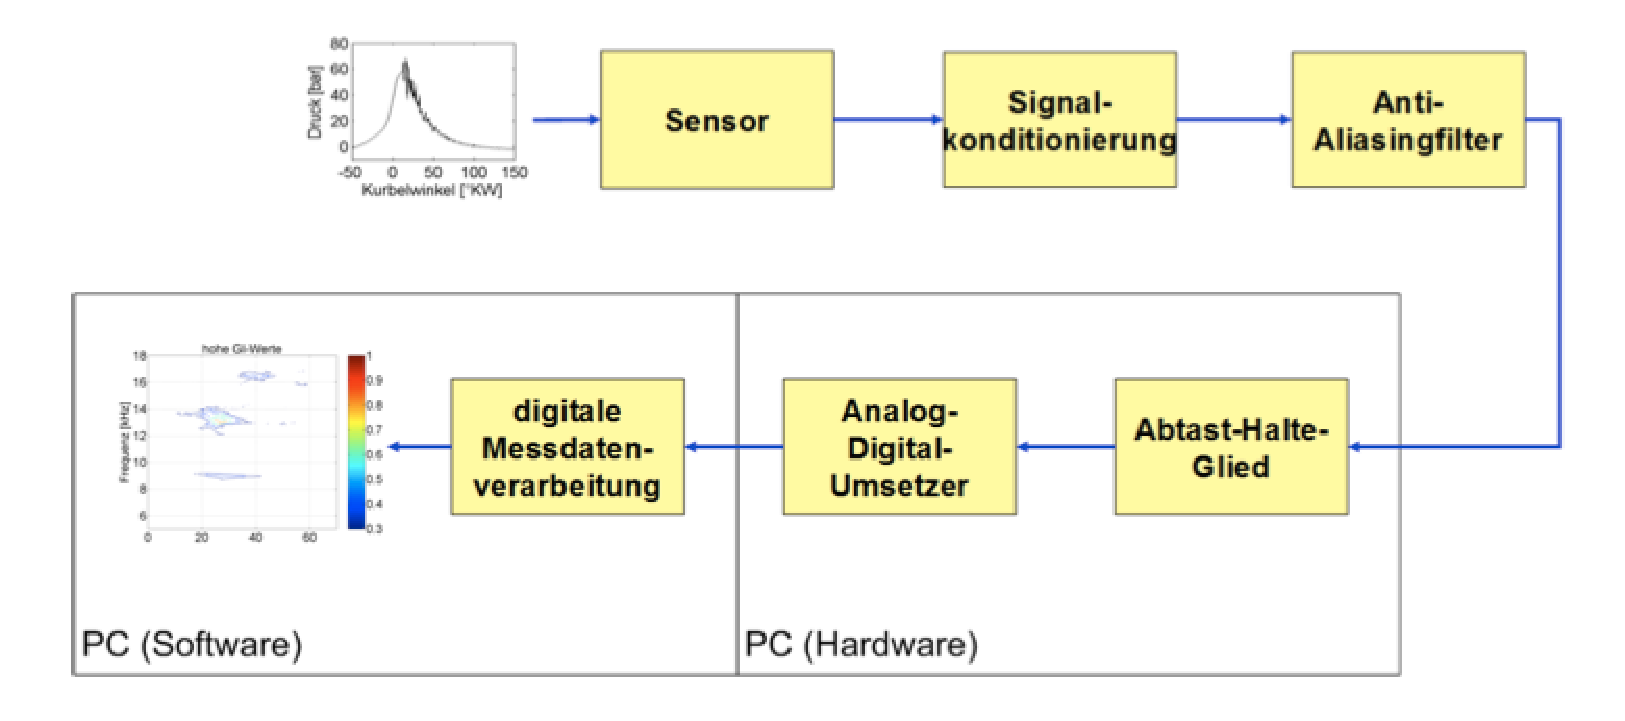
\includegraphics[scale=0.5]{DigitaleMesskette}
				   \caption{Digitale Messkette}
		\cite{DigitaleMesskette}
		\end{figure}
		\vspace{1em}
	 	
	 	Wir betrachten einige dieser Bauteile etwas genauer:
	 	\subsubsection{Signalkonditionierung}
		\begin{quote}
			Die Signalkontitioniertung hat das Ziel das Signal des Sensors an den Aussteuerbereich des Messystems anzupassen. Das
			kann bedeuten, dass das Signal verstärkt, gedämpft, gefiltert, linearisiert oder konvertiert werden muss. 
		\end{quote}
		\subsubsection{Anti-Aliasingfilter}
		\begin{quote}
		      Beim Abtasten eines Signals entsteht ein periodisches Spektum.Der Anti-Aliasingfilter hat die Aufgabe alle
		      Frequenzen die größer als die halbe Abtastfrequenz sind zu unterdrücken. 
		      
		      \begin{equation*}
                	\begin{split}
                		\omega > \frac{\omega_0}{2} \hspace{2em} \text{mit} \hspace{2em} \omega_0 = \frac{2\pi}{T}
                	\end{split}
                \end{equation*}
		      
		      Hierzu werden alle zu hohen Frequenzen von ihrer Amplitude auf einen Wert unterhalb des
              \" least significant bits \" gedämpft.\\
		      
		      Würden diese Frequenzen nicht gefiltert werden würde es zu dem sogenannten Aliasing kommen bei dem höhere
		      Frequenzanteile fälschlicherweise als kleinere Frequenzen interpretiert werden. Als folge würde das
		      Originalsignal verfälscht weitergeleitet.\\
		      
		      Da ein abgetastetes Signal umso mehr dem Originalsignal ähnelt je höher die Abtastfrequenz ist, ist in diesem
		      Sinne eine möglichst hohe Abstastfrequenz erstrebenswert. Eine höhe Abstastfrequenz hat jedoch zur folge, dass
		      ein steilerer Anti-Aliasingfilter notwendig ist um das Aliasing zu verhindern. Außerdem ist die
		      Schaltungstechnische Umsetzung bald sehr herausfordernd.\\
		      Des weiteren begrenzt der Analog-Digital-Umsetzer die minimale Abtastfrequenz, da der ADU eine gewisse Zeit
		      benötigt um ein Signal umzuwandeln. Es ergibt keinen Sinn ein Signal Häufiger abzutasten als der ADU umwandeln
		      kann.
		\end{quote}
		\subsubsection{Abtast-Halte-Glied}
        \begin{quote}
            Ein Abtast-Halte-Glied hat die Aufgabe einen Wert abzutasten und für die zeit zu halten die der ADU
            benötigt um aus dem Abgetasteten analogen Wert ein digitalen Wert zu konvertieren.
        \end{quote}
        \subsubsection{ADU}
		\begin{quote}
			Der Analog-Digital-Umsetzer ermittelt aus dem abgetasteten analogen Signal das dazupassende Digitale Signal.\\
		\end{quote}
		
		In dem praktischen Aufbau werden der Sensor sowie die Signalkonditionierung durch die Spannungsquelle realisiert.
		Die externe Wandler-Box übrnimmt die Aufgabe des Anti-Aliasingfilters. Auf dem Micro-Controller selbst ist das
		Abstast-Halte-Glied sowie der Analog-Digital-Umwandler integriert.
    \end{quote}
    
    \subsection{Berechnung der Abtastfrequenz bei einem Butterworth-Tiefpass 2.Ordnung}
    \begin{quote}
        Gegeben ist ein Tiefpass 2.Ordnung mit einer $3dB$-Grenzfrequenz von $f_g=3,1kHz$. Wir wählen einen
        Butterworthtiefpass und erstellen den Frequenzgang.\\
        Die Übertragungsfunktion eines Tiefpasses 2. Ordnung lautet:
        
        \begin{equation*}
        	\begin{split}
        		H(j\omega) = \frac{1}{1 + \frac{\sqrt{2}}{f_g 2 \pi}j\omega + \frac{1}{(f_g 2 \pi)^2}(j\omega)^2}
        	\end{split}
        \end{equation*}
        
        Daraus ergibt sich folgender Frequenzgang:
        
        \begin{figure}[H]
			\centering
				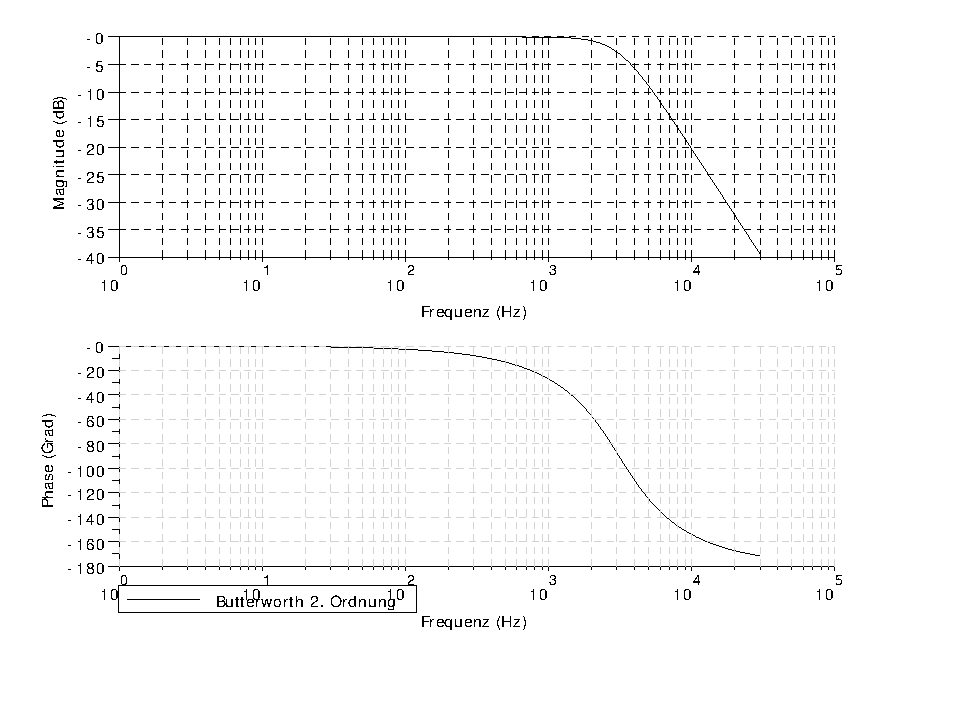
\includegraphics[scale=1]{Frequenzgang}
				   \caption{Frequenzgang Butterworthtiefpass 2. Ordnung}
		\end{figure}
		\vspace{1em}
	 	
	   Als nächstes berechnen wir die benötigte Dämpfung, die das Aliasing verhindert. Dazu dämpfen wir die maximal
	   mögliche Amplitude auf einen kleineren Wert als $U_{LSB}$. In unserem Fall ist der Spannungsbereich von $-7V$-$+7V$
	   bei einem $10Bit$ ADU. Daraus ergibt sich folgendes \"least significant bit\"
	   
	   \begin{equation*}
        	\begin{split}
        		U_{LSB} = \frac{(7V-(-7V))}{2^{10}-1} = \frac{14}{1023}
        	\end{split}
        \end{equation*}
        
        Daraus ergibt sich, dass eine maximale Amplitude von $+7V$ um einen Wert von $\frac{2}{1023}$ bzw. $10
        Log(\frac{2}{1023}) = -27 dB$ gedämpft werden muss. \\
        An dem Frequenzgang sehen wir, dass alle Frequenzen die größer sind als $20kHz$ um mehr als $-30 dB$ gedämpft
        werden. Aus diesem Wissen ergibt sich, dass die Abtastfrequenz $f_0 = 40kHz$ betragen soll.
        
    \end{quote}
    
    \subsection{Berechnung der Abtastfrequenz bei einem Butterworth-Tiefpass 8.Ordnung}
    \begin{quote}
        Die neue Übertagungsfunktion $H_2$ des Tiefpasses 8. Ordnung
        
        \begin{equation*}
        	\begin{split}
        		H_2(j\omega) = H^4 (j\omega)
        	\end{split}
        \end{equation*}
        
        Daraus ergibt sich nun der folgende Frequenzgang:
        
        \begin{figure}[H]
			\centering
				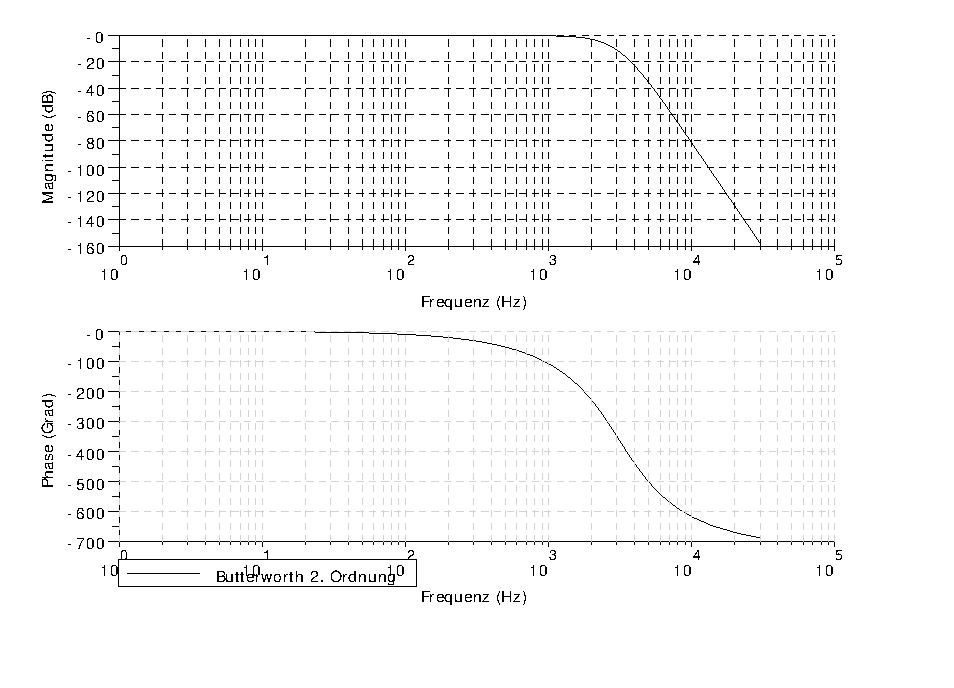
\includegraphics[scale=1]{Frequenzgang8Ordnung}
				   \caption{Frequenzgang Butterworthtiefpass 8 Ordnung}
		\end{figure}
		\vspace{1em}
	 	
	 	Da sich die Bedingung der Dämpfung nicht geändert hat kontrollieren wir ab welcher Frequenz bei diesem aktuellen
	 	Frequenzgang eine Dämpfung von mindestens $-27 dB$ erreicht wird.\\
	 	Bei Frequenzen größer als $5kHz$ ist die Dämpfung größer als $-36 dB$. Daraus ergibt sich eine neue Abtastfrequenz
	 	von $f_0 = 10kHz$.
    \end{quote}
    
    \section{Spektralanalyse}
    \begin{quote}
    	Um ein $2kHz$ Signal abzutasten, würde eine Abtastfrequenz von wenigstens $4 kHz$ ausreichen. Allerdings würde
    	hierbei Aliasing auftreten, da der Tiegpassfilter eine Grenzfrquenz von $3,1kHz$ hat.\\
    	Aus diesem Grund benutzen wir die in der vorigen Aufgabe ausgerechnete Abtastfrequenz von $10kHz$.
    \end{quote}
\end{quote}

%--------------------------------------------------------------------
%--------------------------------------------------------------------

\section{Versuch}
\begin{quote}
	
\end{quote}

%--------------------------------------------------------------------
%--------------------------------------------------------------------

\section{Ergebnisse}
\begin{quote}
	
\end{quote}

%--------------------------------------------------------------------
%--------------------------------------------------------------------

\begin{thebibliography}{999}
\bibitem {DigitaleMesskette} Prof. Dr.-Ing. Gühmann, Clemens: MDVScript\_01, S.5

%Name, Vorname.; evtl. Name2, Vorname2.: Titel des Dokumentes
%oder Buches, Zeitschrift/Verlag/URL (Auflage, Erscheinungsort, -jahr), ggf. Seitenzahlen
%\bibitem [Wiki10] {DigitaleMesskette2} \url{www.wikipedia.org}, Zugriff 22.03.2010
\end{thebibliography}


\end{document}


